
\section{Classification}

\begin{breakbox}
\boxtitle{Terms \& Definitions:}
\newline Instances:
\begin{itemize}
	\item also: samples, examples, records, tuples, objects.
	\item individual, independent samples, e.g. a customer transaction.
\end{itemize}
 Attributes:
\begin{itemize}
	\item qualities, properties of instances (e.g. profession, age, education etc.).
\end{itemize}
 Attribute value:
\begin{itemize}
	\item concrete occurrence of an attribute (e.g. IT analyst, 37, master in computer science).
\end{itemize}
Class label (class attribute):
\begin{itemize}
	\item attribute determining the class of an instance (e.g. potential customer).
\end{itemize}
Class:
\begin{itemize}
	\item distinct value of the class label (e.g. yes).
\end{itemize}
\end{breakbox}

\begin{breakbox}
\boxtitle{1R Algorithm:}
\begin{center}
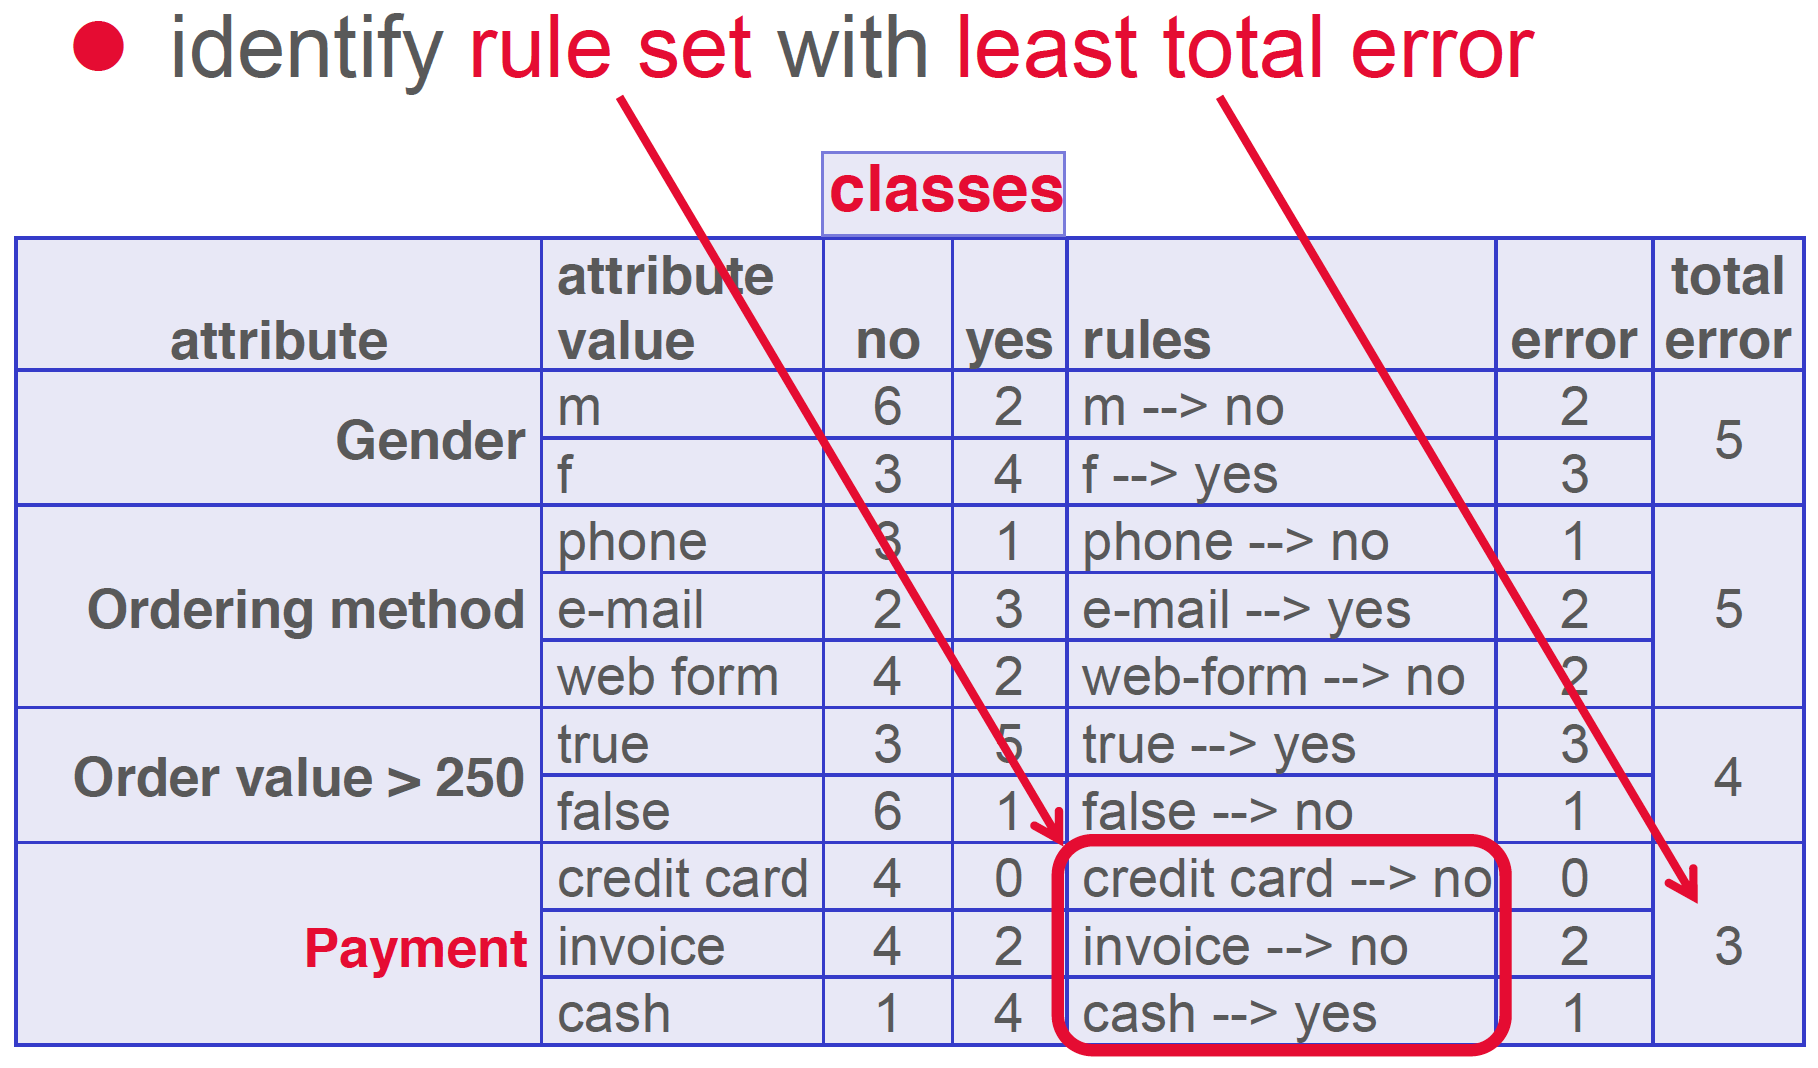
\includegraphics[width=.15\textwidth]{slides_images/1r_algorithm}
\end{center}
\end{breakbox}

\begin{breakbox}
\boxtitle{ID3-Algorithm:}
\begin{enumerate}
	\item Start with root node where no attribute is assigned yet. Root node contains full set of training instances.
	\item Identify individual classes and determine distribution of classes over instances.
	\item Calculate information content of current node (see below).
	\item Choose remaining attribute (not examined yet on path between current node of tree and root node). If no attributes left $\rightarrow$ exit.
	\item Determine attribute's value domain. Create preliminary child node for each distinct value.
	\item Partition set of instances (i.e. assign them to individual child nodes).
	\item Determine distribution of classes for each partition (child node).
	\item Calculate entropy of child nodes (see below).
	\item Calculate information gain (see below).
	\item If attributes left for examinig $\rightarrow$ go to 4.
	\item Select attribute with highest information gain. Insert it into current tree node. This attribute will not be considered any more in dependent sub-trees.
	\item Append attribute's child nodes to current tree node.
	\item Go to leftmost child node which is neither leaf nor has fully developed subtree structure. If there is none $\rightarrow$ go to next sibling node which is no leaf. If there is none either $\rightarrow$ go to parent node. If parent node is root node $\rightarrow$ exit, else repeat 13.
	\item Go to 4.
\end{enumerate}

\begin{breakbox}
\boxtitle{Calculate information content:}
\begin{center}
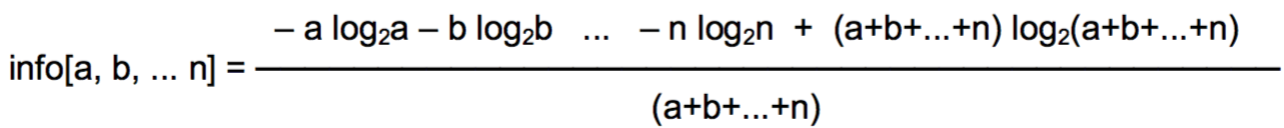
\includegraphics[width=.15\textwidth]{slides_images/information_content}
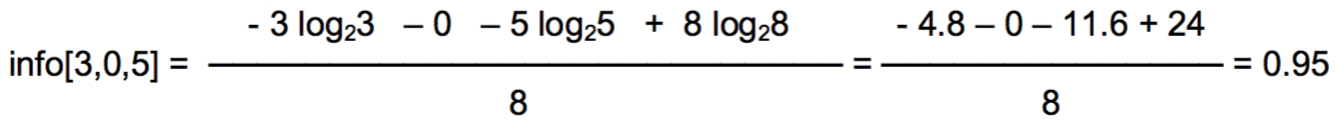
\includegraphics[width=.15\textwidth]{slides_images/information_content_example}
\end{center}
\end{breakbox}

\begin{breakbox}
\boxtitle{Calculate entropy:}
\begin{center}
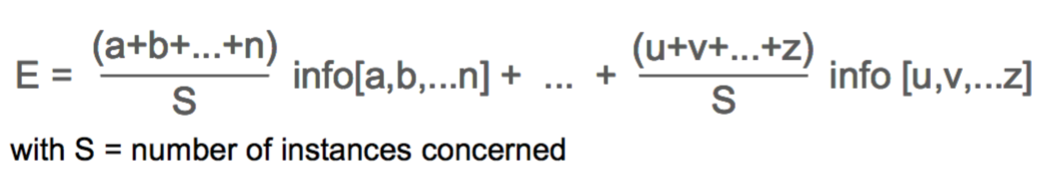
\includegraphics[width=.15\textwidth]{slides_images/entropy}
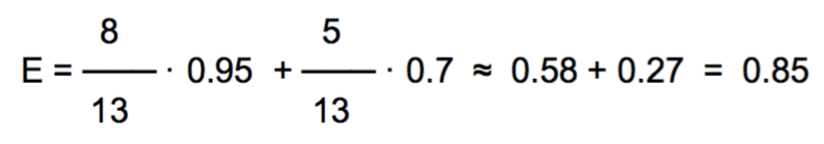
\includegraphics[width=.15\textwidth]{slides_images/entropy_example}
\end{center}
\end{breakbox}

\begin{breakbox}
\boxtitle{Calculate information gain:}
\newline Gain = info[parent node] - E[child node]
\end{breakbox}

\begin{center}
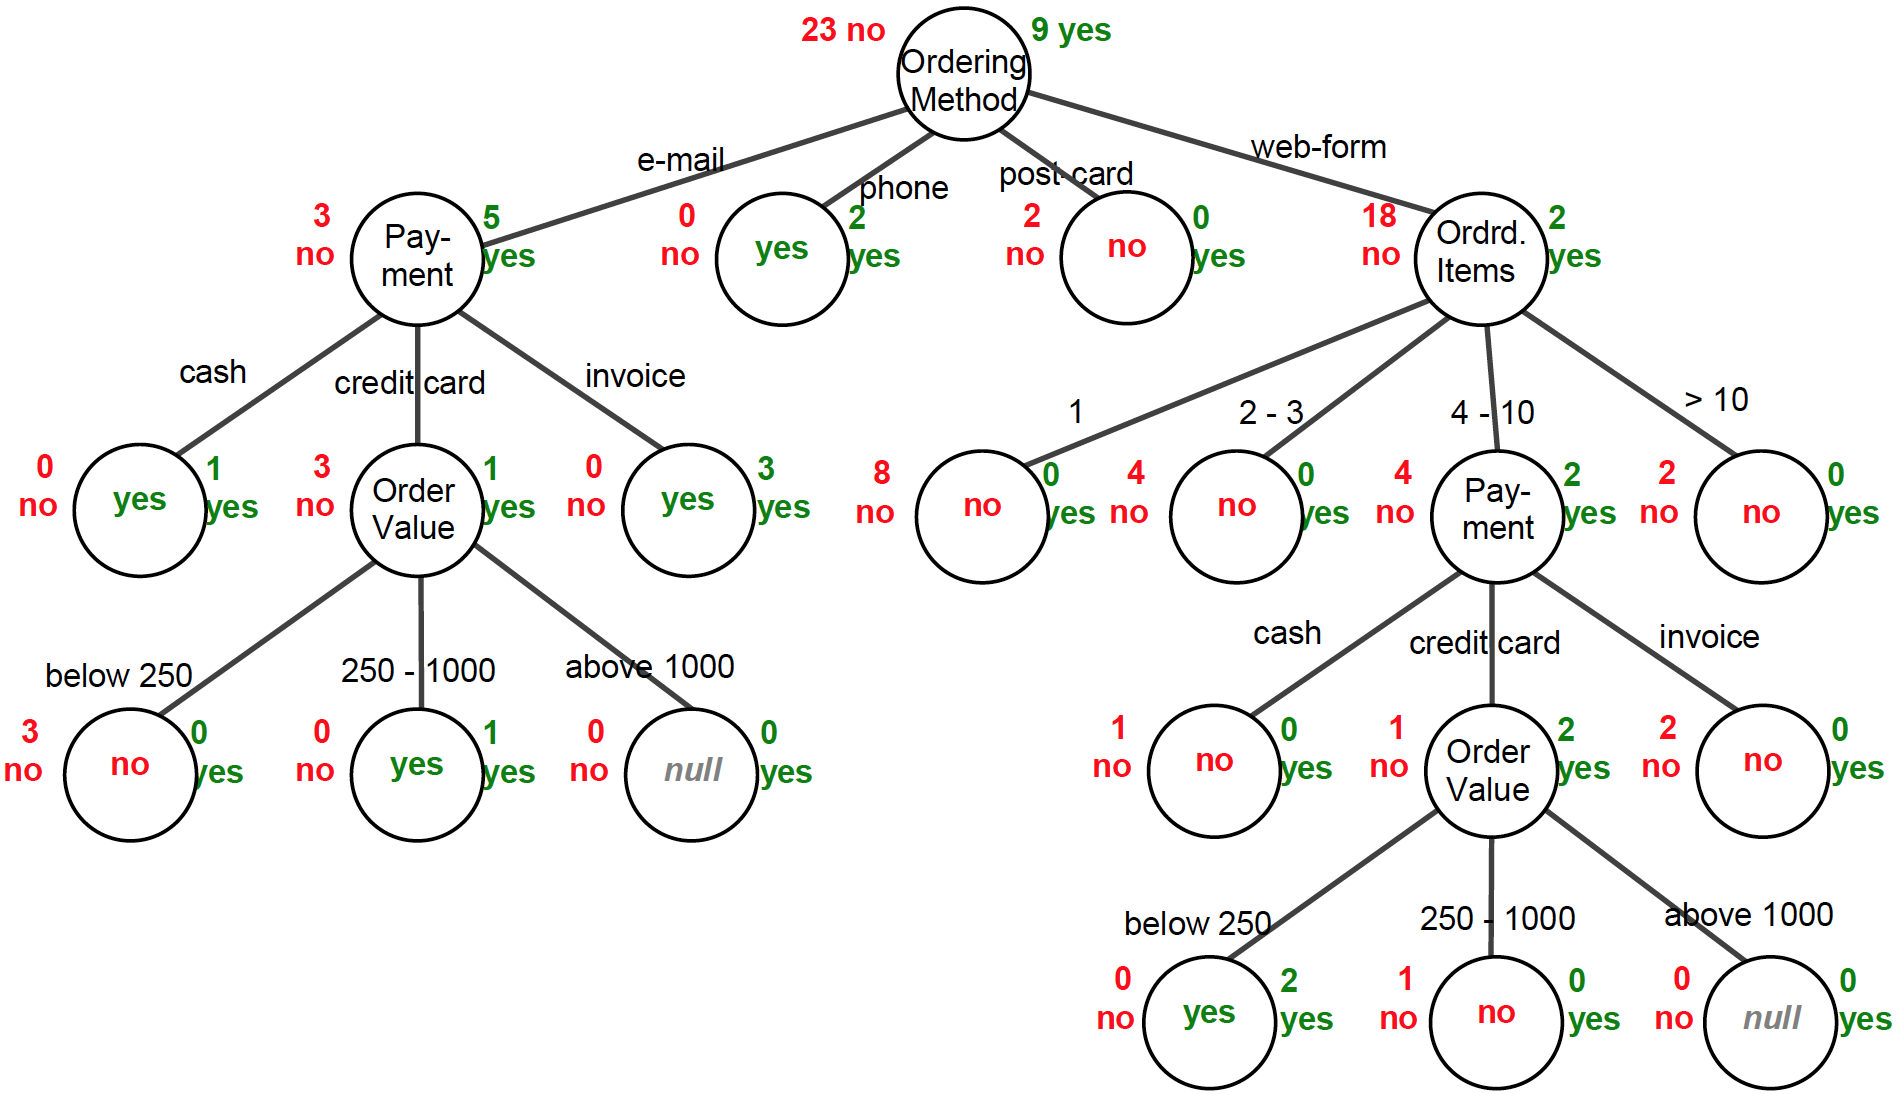
\includegraphics[width=.15\textwidth]{slides_images/id3_tree}
\end{center}

%\begin{breakbox}
%\boxtitle{Approximate values for $x log_2(x)$:}
%\begin{center}
%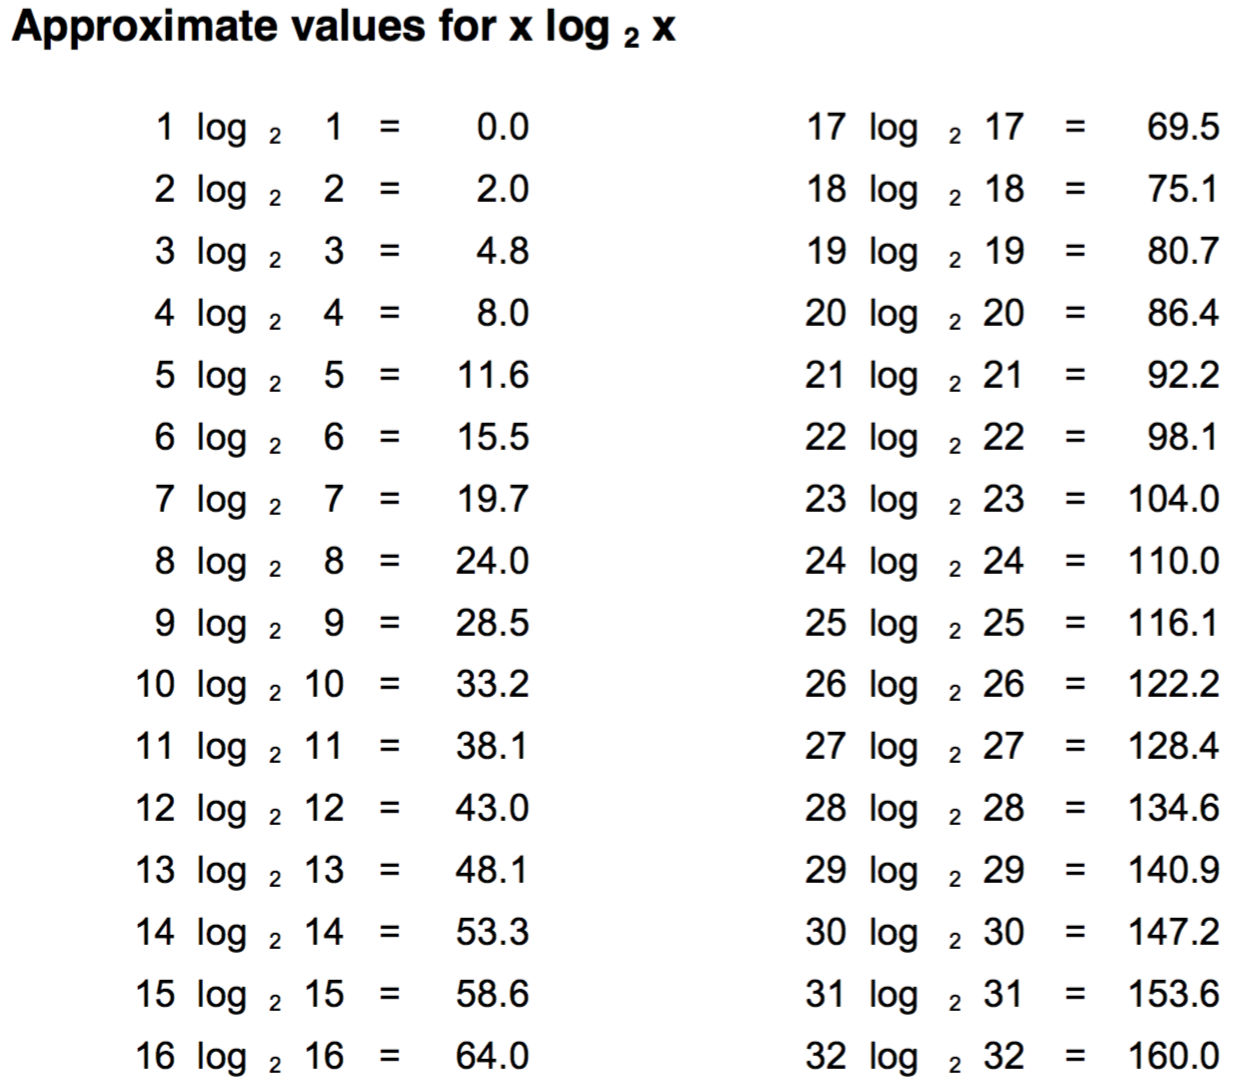
\includegraphics[width=.15\textwidth]{slides_images/log_values}
%\end{center}
%\end{breakbox}
\end{breakbox}

\begin{breakbox}
\boxtitle{Naïve Bayes:}
\newline \textcolor{Emerald}{A-Priori Probability:}
\begin{itemize}
	\item P(Newly industrialized country) = 5/25
	\item P(Developing country) = 8/25
\end{itemize}
\textcolor{Emerald}{A-Posteriori Probability:}
\begin{center}
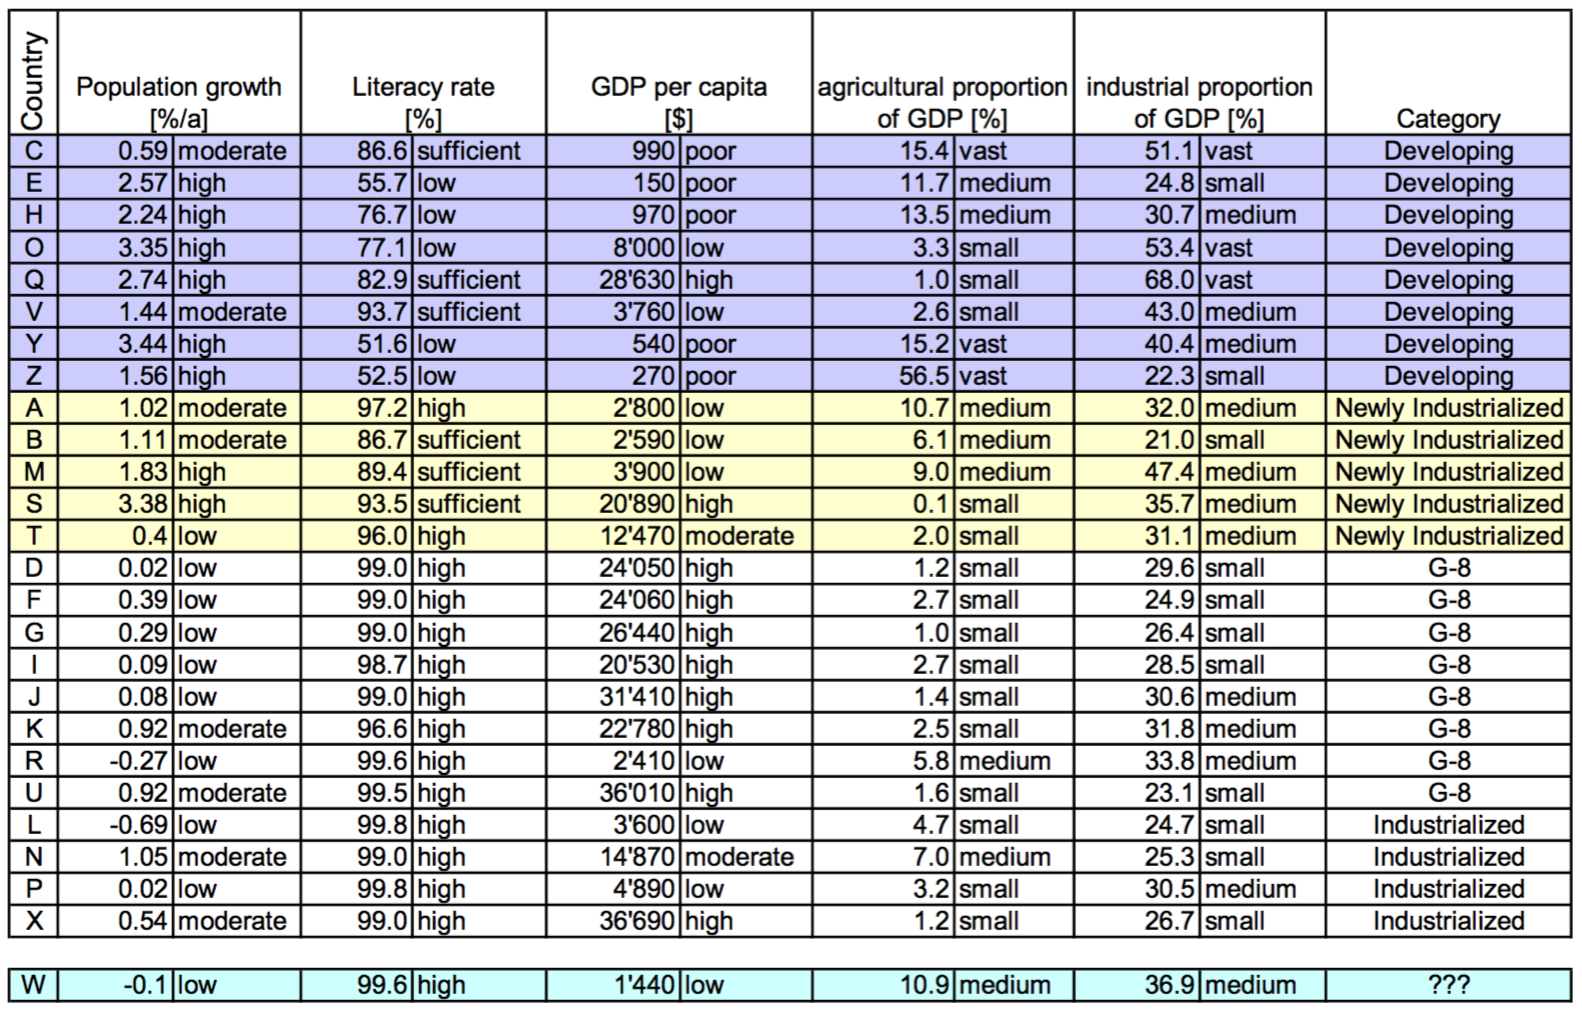
\includegraphics[width=.15\textwidth]{slides_images/naive_bayes_table}
\end{center}
For P(Country W | Newly industrialized country):
\begin{itemize}
	\item Population growth: low $\rightarrow$ 1/5 = 0.2
	\item Literacy: high $\rightarrow$  2/5 = 0.4
	\item GDP/capita: low $\rightarrow$ 3/5 = 0.6
	\item Agricultural GDP: medium $\rightarrow$ 3/5 = 0.6
	\item Industrial GDP: medium $\rightarrow$ 4/5 = 0.8
\end{itemize}
For P(Country W | Developing country):
\begin{itemize}
	\item Population growth: low $\rightarrow$ 0
	\item Literacy: high $\rightarrow$  0
	\item GDP/capita: low $\rightarrow$ 2/8 = 0.25
	\item Agricultural GDP: medium $\rightarrow$ 2/8 = 0.25
	\item Industrial GDP: medium $\rightarrow$ 4/5 = 0.375
\end{itemize}
\textcolor{Emerald}{Probability for specific category:}
\newline P(Country W | Newly industrialized country) $\cdot$ P(Newly industrialized country):
\begin{itemize}
	\item $0.2 \cdot 0.3 \cdot 0.6 \cdot 0.6 \cdot 0.8 \cdot 0.2 = 4.608 \cdot 10^{-3}$
\end{itemize}
P(Country W | Developing country) $\cdot$ P(Developing country):
\begin{itemize}
	\item $0.0909 \cdot 0.0909 \cdot 0.25 \cdot 0.25 \cdot 0.375 \cdot 0.32 = 0.062 \cdot 10^{-3}$
	\item Note: We pretend having had at least 1 occurrence for each of the non-occuring attributes. In return we add 1 fictious occurence for the other attributes as well. Of course, when doing so we have to increase the total number of instances accordingly (1/11 = 0.0909 for first to attributes).
\end{itemize}
So country W is definitely a newly industrialized country (at least according to Bayes).
\end{breakbox}
























